\section{Finding high-growth sequences}
\label{sec:dualalgo}
In \secref{sos}, we introduced the SOS restriction of \progref{primalinf} with \progref{primal}.
In this section, we introduce \progref{dual}, the moment relaxation of \progref{dualinf}.
It turns out that \progref{primal} and \progref{dual} are dual to each other.
Indeed, the proof of \lemref{duality} can be translated verbatim in order to prove that \progref{dual} is the dual of \progref{primal}.


\subsection{Dual SOS program}
\label{sec:dual}




\begin{myprog}[Dual of \progref{primal}]
  \label{prog:dual}
  \begin{align}
    \notag
    \sup_{\pmu_{uv\sigma} \in \Rhd, \gamlb \in \R} \gamlb\\
    \label{eq:dual1}
    \sum_{(u,v,\sigma) \in \Arcs} \pushf{A_\sigma}{\pmu_{uv\sigma}} - \gamlb^{2d} \sum_{(v,w,\sigma) \in \Arcs} \pmu_{vw\sigma} & \in \Soshd, \forall v \in \Nodes,\\
    \label{eq:dual2}
    \pmu_{uv\sigma} & \in \Soshd, \quad \forall (u,v,\sigma) \in \Arcs,\\
    \label{eq:dual3}
    \sum_{(u,v,\sigma) \in \Arcs} \pmu_{uv\sigma}(\Sn) & = 1.
  \end{align}
\end{myprog}





It is important to note that a solution of \progref{dual} is not necessarily a solution of \progref{dualinf}.
First $\pmu_{uv\sigma}$ may not be a measure even if it belongs to $\Soshd$ as discussed in \secref{sosprog}.
Second, the left-hand side of \eqref{eq:dual1} may also not be a measure.
For this second concern, it helps to be more explicit.
Suppose for instance that we are in the quadratic case, i.e. $d = 1$.
In that case, if $\pmu \in \Soshd[2]$, there always exists a measure $\mu$ that has the moments of the pseudo-measure $\pmu$.
We can take for instance a Gaussian distribution with these second order moments.
Hence we can find Gaussian distributions $\mu_{uv\sigma}$ that have the second order moments $\pmu_{uv\sigma}$
and Gaussian distributions $\nu_v$ that have the second order moments given by the left-hand side of \eqref{eq:dual1}.
However, we may have
\[ \sum_{(u,v,\sigma) \in \Arcs} \pushf{A_\sigma}{\mu_{uv\sigma}} - \gamlb^{2d} \sum_{(v,w,\sigma) \in \Arcs} \mu_{vw\sigma} \neq \nu_v \]
as we only know that the left-hand side and right-hand side of the above equation have the same second order moments;
see \exemref{run3}.

However, in some cases, we can recover a feasible solution of \progref{dualinf} from a feasible solution of \progref{dual}.
In these cases, by \cororef{instabcert}, this provides a lower bound on the CJSR.
Moreover, there exist efficient techniques allowing to detect situations where the solution is moments of an atomic measure; see \cite{henrion2005detecting, laurent2009sums}.
Then, using the transformation of \propref{Bsc}, we can transform
these atomic measures into a feasible solution of a constrained scalar switched systems.
For such system, we could use the algorithm described in \lemref{instabcerts} but as pointed out in \cite{ahmadi2012joint},
computing the CJSR of a scalar system can easily be done by solving a maximum cycle mean problem for which efficient algorithm exists \cite{karp1978characterization}.

If we recover a feasible solution of \progref{dualinf} from a feasible solution of \progref{dual} with $\gamlb = \jsrsos$,
we can directly conclude that $\jsrsos = \cjsr$.
This is somewhat similar to the minimization of a multivariate polynomial using SOS where we can detect that we have reached the optimum
when the measure is atomic and recover the minimizers of the polynomial from the atoms of the measure. %

However, we may also check for atomic feasible solutions of \progref{dualinf} with $\gamlb < \jsrsos$ to provide lower bounds.
Moreover, in practice, $\jsrsos$ is computed by binary search on $\gamlb$ so we often have several such solutions.

\begin{myexem}
  \label{exem:simple2}
  Consider \exemref{simple1}.
  For $i = 1, 2, 3$, let $\pmu_i$ be the solution of \progref{dual} corresponding to the matrix $A_i$.
  For any $d$, we can see that the dual solution for $\gamma = 1$ is such that
  the only monomial $x^\alpha$ such that $\la\pmu_1, x^\alpha \ra$ (resp. $\la \pmu_2, x^\alpha \ra$, $\la \pmu_3, x^\alpha \ra$) is non-zero is $x_1^{2d}$ (resp. $x_2^{2d}$, $x_3^{2d}$)
  and $\la \pmu_1, x_1^{2d} \ra = \la \pmu_2, x_2^{2d} \ra = \la \pmu_3, x_3^{2d} \ra = 1/3$.
  Note that it means that $\pmu_1 = \delta_{(1,0,0)}/3$, $\pmu_2 = \delta_{(0,1,0)}/3$ and $\pmu_3 = \delta_{(0,0,1)}/3$
  where $\delta_x$ is the Dirac measure centered on $x$.
  Since these measures are solution to \progref{dualinf} with $\gamlb = 1$,
  by \cororef{instabcert}, this means that $\jsr \geq 1$.
\end{myexem}


\begin{myexem}
  \label{exem:run3}
  We continue the running example; see Example~\ref{exem:run1} and Example~\ref{exem:run2}.

  For all $d$, $\pmu_{212} = \pmu_{323} = \pmu_{344} = \pmu_{431} = 0$
  hence the node 4 is ``unused'' by the dual.
  For $2d = 2, 4$, $\pmu_{123} = \pmu_{231} = 0$ so
  the node $2$ is ``unused'' for low degree.

  At first, one could think that the dual variables can be used to reduce the systems,
  e.g. remove nodes or edges.
  However, it would be a mistake to remove the node 2 since the periodic trajectory with highest growth rate uses this node.



  It is also interesting to notice that the matrices corresponding to the dual variables have low rank.
  For example, for $2d = 2$, $\pmu_{131}$
  (resp. $\pmu_{312}$, $\pmu_{331}$) is the Dirac measure $5.873 \cdot \delta_{(0.917,0.399)}$
  (resp. $3.966 \cdot \delta_{(0.875,0.485)}$, $6.704 \cdot \delta_{(0.757,-0.653)}$).
  However, this is not a feasible solution of \progref{dualinf}.
  Indeed,
  while \eqref{eq:dualinf1} is satisfied for \node{} 1 since
  $\pushf{A_2}{\delta_{(0.875,0.485)}}$ gives $\delta_{(0.917,0.399)}$,
  \eqref{eq:dualinf1} is not satisfied for \node{} 3 as
  $\pushf{A_1}{\delta_{(0.917,0.399)}}$ gives $\delta_{(0.999, -0.0271)}$ and
  $\pushf{A_1}{\delta_{(0.757,-0.653)}}$ gives $\delta_{(0.422, -0.906)}$.
\end{myexem}


\subsection{Generating high growth sequence}
\label{sec:algo}
In this section we give an algorithm that generates an infinite
sequence of matrices such that the asymptotic growth rate of the
product of the matrices is arbitrarily close to the CJSR.
Note that by \defref{cjsr}, this asymptotic growth rate must be
smaller than the CJSR.


Given an \arc{} $e \in \Arcs$, let $\pE_e[p(x)] = \la \pmu_e, p(x) \ra$.
Given a polynomial $p_0(x) \in \inte(\Sosh)$ and an initial edge $(v_1,v_0,\sigma_1)$,
the algorithm builds a $\G^\Tr$-admissible
sequence $(v_1,v_0,\sigma_1),\allowbreak(v_2,v_1,\sigma_2), \ldots$ such that
\begin{equation}
	\label{eq:thetak}
  \theta_k \eqdef \pE_{v_{k}v_{k-1}\sigma_k}[p_0(A_{\sigma_1} \cdots A_{\sigma_k}x)]
\end{equation}
remains ``large'' for increasing $k$.
As we will see, using \lemref{thetatoA},
this implies that $A_{\sigma_1} \cdots A_{\sigma_k}$ has a ``large'' norm.

\begin{lemma}[{\cite[Lemma~6]{legat2016generating}}]
  \label{lem:sosbound}
  For any polynomial $p(x) \in \inte(\Sosh)$,
  there exists a constant $\beta$
  such that for any matrix $A$,
  \[ \beta\|A\|_2^{2d} p(x) - p(Ax) \quad \text{is SOS} \]
  where $\|A\|_2 = \rho(A^\Tr A)^{1/2}$ is the Euclidean norm.
\end{lemma}

\begin{lemma}
  \label{lem:thetatoA}
  Let us consider a solution $(\, \pmu_e : e \in \Arcs \,)$ of \progref{dual}.
  For any polynomial $p(x) \in \inte(\Sosh)$,
  there exists a positive constant $\tau$
  such that for any matrix $A \in \R^{n \times n}$ and \arc{} $e \in \Arcs$,
  \[ \pE_e[p(A x)] \leq \tau \|A\|_2^{2d} \]
  \begin{proof}
    If all pseudo-expectations are zero, the result is trivially true.
    Therefore we can suppose that at least one is nonzero.
    By \lemref{sosbound}, there exists a constant $\beta > 0$ such that
    \[ \beta \|A\|_2^{2d}p(x) - p(Ax) \text{ is SOS}. \]
    Hence
    \[
      \pE_e[p(Ax)] \leq \beta \|A\|_2^{2d} \pE_e[p(x)].
    \]
    We obtain the result with the constant
    \(
    \tau = \beta \max_{e \in \Arcs} \pE_{e}[p(x)].
    \)
    Since at least one pseudo-expectation is nonzero and $p(x)$ is in
    the interior of the SOS cone, $\tau > 0$.
  \end{proof}
\end{lemma}



\begin{algorithm}[!ht]
  \caption{Generates a sequence of large asymptotic growth using paths of length $l$.}
  \label{algo:prodl}
  \begin{algorithmic}
    \STATE{Given a feasible solution $(\, \pmu_e : e \in \Arcs \,)$ of \progref{dual}}
    \STATE{Pick an arbitrary polynomial $p_0(x) \in \inte(\Sosh)$}
    \STATE{Pick an \arc{} $(v_0,v_{-1},\sigma_0) \in \Arcs$ such that $\pE_{v_0v_{-1}\sigma_0}[p_0(x)] > 0$}
    \FOR{$k = 0,l,2l,\ldots$}
    \STATE Pick $s \in \argmax_{s \in \Arcsin_l(v_{k})} \pE_{s[1]}[p_k(A_s x)]$
    \STATE Set $(v_{k+l},\sigma_{k+l},\ldots,\sigma_{k+1},v_k) \leftarrow s$
    \STATE Set $p_{k+1} \leftarrow p_k(A_s x)$
    \ENDFOR
  \end{algorithmic}
\end{algorithm}





\lemref{maxdegpathl} provides a guarantee on the growth rate of $\theta_k$, defined in \eqref{eq:thetak},
using the dual constraint~\eqref{eq:dual1}.

\begin{lemma}
  \label{lem:dualconsl}
  Given \defAG{}, %
  if $\pmu$ is a feasible solution of \progref{dual} then,
  for any edge $(\bar{u},\bar{v},\bar{\sigma}) \in \Arcs$,
  the following holds:
  \begin{equation}
    \label{eq:dualconsl}
    \sum_{s \in \Arcsin_k(\bar{u})} \pushf{A_s}{\pmu_{s[1]}} \succeq \gamma^{2dk} \pmu_{\bar{u}\bar{v}\bar{\sigma}}
  \end{equation}
  where $\pmu_1 \succeq \pmu_2$ denotes $\pmu_1 - \pmu_2 \in \Soshd$.
  \begin{proof}
    We prove \eqref{eq:dualconsl} by induction, the case of $k=0$ being trivial.
    Suppose that
    \begin{equation}
      \label{eq:indhyp}
      \sum_{s' \in \Arcsin_{k-1}(\bar{u})}\pushf{A_{s'}}{\pmu_{s'[1]}} \succeq \gamma^{2d(k-1)} \pmu_{\bar{u}\bar{v}\bar{\sigma}}.
    \end{equation}
    We can rewrite the left-hand side of \eqref{eq:dualconsl} as
    \begin{equation}
      \label{eq:splitdualconsl}
      \sum_{s \in \Arcsin_k(\bar{u})} \pushf{A_s}{\pmu_{s[1]}} = \sum_{s' \in \Arcsin_{k-1}(\bar{u})} \pushf{A_{s'}}{\sum_{(u,s'(1),\sigma) \in \Arcs} \pushf{A_\sigma}{\pmu_{us'(1)\sigma}}}.
    \end{equation}
    By \eqref{eq:dual1},
    \[
      \sum_{(u,s'(1),\sigma) \in \Arcs} \pushf{A_{\sigma}}{\pmu_{us'(1)\sigma}}
      \succeq \gamma^{2d} \sum_{(s'(1),w,\sigma') \in \Arcs} \pmu_{s'(1)w\sigma'}.
    \]
    Since the dual variables $\pmu_{s'(1)w\sigma'}$ of the right-hand side are in the dual of the SOS cone,
    and one of them is $\pmu_{s'[1]}$, we have
    \[
      \sum_{(u,s'(1),\sigma) \in \Arcs} \pushf{A_{\sigma}}{\pmu_{us'(1)\sigma}}
      \succeq \gamma^{2d} \pmu_{s'[1]}.
    \]
    Applying $\pushf{A_{s'}}{}$ on both sides and using \eqref{eq:splitdualconsl} gives
    \[
      \sum_{s \in \Arcsin_k(\bar{u})} \pushf{A_s}{\pmu_{s[1]}} \succeq \gamma^{2d} \sum_{s' \in \Arcsin_{k-1}(\bar{u})}\pushf{A_{s'}}{\pmu_{s'[1]}} \stackrel{\eqref{eq:indhyp}}{\succeq} \gamma^{2dk} \pmu_{\bar{u}\bar{v}\bar{\sigma}}.
    \]
  \end{proof}
\end{lemma}

\begin{lemma}
  \label{lem:maxdegpathl}
  Consider \defAGe{}.
  For any positive integers $d$ and $l$,
    using \progref{dual} with any $\gamma < \jsrsosa\\(\G,\A)$,
  \algoref{prodl} with paths of length $l$
  produces a $\G^\Tr$-admissible sequence
  $(v_1,v_0,\\\sigma_0),(v_2,v_1,\sigma_1), \ldots$ %
  for which the sequence of $\theta_k$ defined in \eqref{eq:thetak}
  satisfies the following inequality for all $k > 0$ multiple of $l$:
  \begin{equation*}
    \theta_{k}
    \geq \frac{\gamma^{2dl}}{\dink[l](v_{k-l+1})}
    \theta_{k-l}
  \end{equation*}
  \begin{proof}
    By \lemref{dualconsl},
    \begin{align*}
      \sum_{s \in \Arcsin_l(v_{k-l+1})} \pE_{s[1]}[p_{k-l}(A_s x)]
      & \geq \gamma^{2dl} \theta_{k-l}.
    \end{align*}
    Since the value of $s$ chosen by \algoref{prodl} maximises $\pE_{s[1]}[p_{k-l}(A_s x)]$,
    the left-hand side of the above inequality is smaller or equal to $\dink[l](v_{k-l+1})\theta_k$.
  \end{proof}
\end{lemma}


\theoref{fourth} translates the guarantee on $\theta_k$ to a guarantee on $A_{\sigma_1} \cdots A_{\sigma_k}$ using \lemref{thetatoA}.

\begin{theorem}
  \label{theo:fourth}
  Consider \defAGe{}.
  For any positive integer $d$ and $l$,
  using \progref{dual} with any $\gamma < \jsrsos$,
  \algoref{prodl} with paths of length $l$
  produces a $\G^\Tr$-admissible sequence
  $(v_1,v_0,\sigma_0), (v_2,v_1,\sigma_1), \ldots$ %
  that satisfies the following inequality for all $k \geq 1$:
  \begin{equation*}
    \lim_{k \to \infty} \|A_{s_k}\|_2^\frac{1}{k} \geq \frac{\gamma}{\|(A(\G)^\Tr)^l\|_\infty^\frac{1}{2dl}}
  \end{equation*}
  where $s_k = (\sigma_k, \ldots, \sigma_1)$.
  \begin{proof}
    By \lemref{maxdegpathl}, for any $k$ multiple of $l$, %
    \begin{equation*}
      \pE_{s_k[1]}[p_0(A_{s_k}x)] \geq \frac{\gamma^{2dk}}{(\mdin_l)^\frac{k}{l}} \pE_{v_0v_{-1}\sigma_0}[p_0(x)]
    \end{equation*}

    By Lemma~\ref{lem:thetatoA},
    there exists a constant $\tau > 0$ such that
    \[
      \pE_{s_k[1]}[p_0(A_{s_k} x)] \leq \tau \|A_{s_k}\|^{2d}.
    \]

    Combining these two inequalities, we obtain
    \begin{align*}
      \tau \|A_{s_k}\|^{2d} & \geq \frac{\gamma^{2dk}}{(\mdin_l)^\frac{k}{l}} \pE_{v_0v_{-1}\sigma_0}[p_0(x)].
    \end{align*}
    Since $\pE_{v_0v_{-1}\sigma_0}$ is nonzero, $\pE_{v_0v_{-1}\sigma_0}[p_0(x)] > 0$.
    Therefore taking the $(2dk)$th root and the limit $k \to \infty$
    we obtain the result.
  \end{proof}
\end{theorem}


Taking the limit $l \to \infty$ and using \eqref{eq:rhoAG}, we see
that Theorem~\ref{theo:second} is a corollary of
Theorem~\ref{theo:fourth}.



\begin{myexem}
  \label{exem:simple3}
  Suppose that we apply Algorithm~\ref{algo:prodl} with $l = 1$ to \exemref{simple2}
  and let us denote by $c_\alpha$ the coefficient of the monomial $x^\alpha$ in the polynomial $p_0(x)$ chosen arbitrarily by the algorithm.
  The start of the sequence produced depends on the order between
  the coefficients $c_{(2d,0,0)},\allowbreak c_{(0,2d,0)},\allowbreak c_{(0,0,2d)}$.
  If $c_{(2d,0,0)}$ is the largest then
  the $\G$-admissible left-infinite sequence found is
  \( \ldots,1,2,3,1,2,3,1,2,3. \)

  The product $A_{\sigma_1} A_{\sigma_2} A_{\sigma_3} \cdots = A_3A_2A_1A_3A_2A_1 \cdots $
  is periodic and has an asymptotic growth rate $\rho(A_{\sigma_1}A_{\sigma_2}A_{\sigma_3})^{1/3}\allowbreak = 1$.
  Hence $1 \leq \cjsr$.
\end{myexem}


\begin{figure}[!ht]
  \begin{subfigure}{0.48\textwidth}
  \centering
    \begin{tikzpicture}
      \SetGraphUnit{1.2}
      \GraphInit[vstyle=Dijkstra]
      \SetVertexNoLabel
      \SetUpEdge[style={->}]
      \Vertex[NoLabel=false,L=$v_k$]{0}
      \NOWE(0){4};
      \NOEA(0){5};
      \SO[NoLabel=false,L=$v_{k-1}$](0){11};
      \tikzset{VertexStyle/.append style = {dashed}}
      \SOWE(0){10};
      \SOEA(0){12};
      \Edge[label=?](4)(0);
      \Edge[label=?](5)(0);
      \Edge(0)(11);
      \tikzset{EdgeStyle/.append style = {dashed}}
      \Edge(0)(10);
      \Edge(0)(12);
    \end{tikzpicture}
    \caption{One iteration of Algorithm~\ref{algo:prodl} with $l = 1$.}
    \label{fig:path1}
  \end{subfigure}
  \begin{subfigure}{0.48\textwidth}
  \centering
    \begin{tikzpicture}
      \SetGraphUnit{1.2}
      \GraphInit[vstyle=Dijkstra]
      \SetVertexNoLabel
      \SetUpEdge[style={->}]
      \Vertex[NoLabel=false,L=$v_k$]{0}
      \NOWE(0){4};
      \NOEA(0){5};
      \NOWE(4){6};
      \NO  (4){7};
      \NOEA(4){8};
      \NOEA(5){9};
      \SO[NoLabel=false,L=$v_{k-1}$](0){11};
      \tikzset{VertexStyle/.append style = {dashed}}
      \SOWE(4){1};
      \EA(0){2};
      \EA(2){3};
      \SOWE(0){10};
      \SOEA(0){12};
      \Edge[label=?](6)(4);
      \Edge[label=?](7)(4);
      \Edge[label=?](8)(4);
      \Edge[label=?](8)(5);
      \Edge[label=?](9)(5);
      \Edge[label=?](4)(0);
      \Edge[label=?](5)(0);
      \Edge(0)(11);
      \tikzset{EdgeStyle/.append style = {dashed}}
      \Edge(4)(1);
      \Edge(5)(2);
      \Edge(5)(3);
      \Edge(0)(10);
      \Edge(0)(12);
    \end{tikzpicture}
    \caption{One iteration of Algorithm~\ref{algo:prodl} with $l = 2$.}
    \label{fig:path2}
  \end{subfigure}
  \caption{Comparison between Algorithm~\ref{algo:prodl} with $l = 1$ and $l = 2$.
  The solid edge denotes the the edge $(v_k, v_{k-1}, \sigma_k)$
  and the edges with question marks denote the incoming path considered by the iteration of the algorithm.}
  \label{fig:paths}
\end{figure}



\subsection{Producing lower bounds}
\label{sec:lb}


By definition of the CJSR, the asymptotic growth rate of the norm of the product of any $\G$-admissible (or $\G^\Tr $-admissible) sequence of matrices gives a lower bound on the CJSR.
In particular the sequence produced by Algorithm~\ref{algo:prodl} provides a lower bound on the CJSR.

If there are two integers $\bar{k},k$ such that the sequence after $\bar{k}$ is periodic of period $k$,
the asymptotic growth rate of the norm is equal to the $k$th root of the spectral radius of the product of the matrices of one period.
This is due to the Gelfand's formula $\rho(A) = \lim_{k \to \infty} \|A^k\|^{1/k}$.
From the same identity,
we see that the spectral radius of the product of the matrices of one $\G$-admissible cycle gives a lower bound on the CJSR.



To find lower bounds for the CJSR,
one could generate all the cycles of length smaller than some maximum length
and compute the spectral radius for all of them.
This brute force approach is not scalable because the number of paths considered grows exponentially with the maximum length.%
\footnote{The exponential growth of the brute force approach is the reason why one should choose a small $l$ for Algorithm~\ref{algo:prodl}.}

Gripenberg~\cite{gripenberg1996computing} proposes a branch-and-bound algorithm that prunes the search using an a priori fixed absolute error.
Two other branch-and-bound variant exists:
the balanced complex polytope algorithm \cite{guglielmi2008algorithm}
and the invariant conitope algorithm~\cite{jungers2014lifted}.

These algorithms can also be used to produce a $\G$-admissible sequence of matrices of high asymptotic growth rate
by reproducing the cycles of high spectral radius infinitely.
The advantage of Algorithm~\ref{algo:prodl} is that it provides a guarantee of accuracy given in \theoref{fourth}.
Algorithm~\ref{algo:prodl} provides at the same time a high growth infinite trajectory and lower bounds of guaranteed accuracy.

We can compute lower bounds using the upper bound provided by Program~\ref{prog:primal} and Corollary~\ref{coro:mix}
but in practice the trajectories are periodic after some time $\bar{k}$ so we are able to compute
much better lower bounds than the pessimistic bound provided by Corollary~\ref{coro:mix}.
This is shown by the following example.

\begin{myexem}
  \label{exem:run4}
  We tried the atom extraction procedure and Algorithm~\ref{algo:prodl} for $l = 1$ and $l = 3$ on our running example;
  see Example~\ref{exem:run1}, Example~\ref{exem:run2} and Example~\ref{exem:run3}.
  The code used to obtain the results of this example can be found on the author's website. %
  The result is shown in \figref{pedj}.
  We showed in \cite{legat2016generating} that the CJSR of the system is equal to 0.97482.
  We can see that this lower bound is found for $d = 4$ for $l=1$ and for $d=1$ for $l=3$.
  The atom extraction finds the lower bound 0.939255.
\end{myexem}

\begin{figure}[!ht]
  \begin{subfigure}{0.48\textwidth}
    \centering
    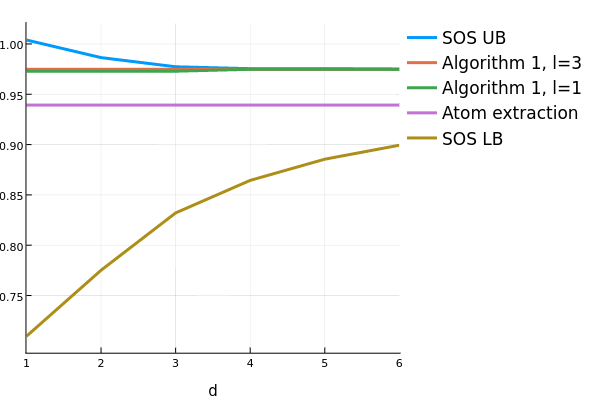
\includegraphics[width=\textwidth]{../../latex/images/PEDJ.png}
  \end{subfigure}
  \begin{subfigure}{0.48\textwidth}
    \centering
    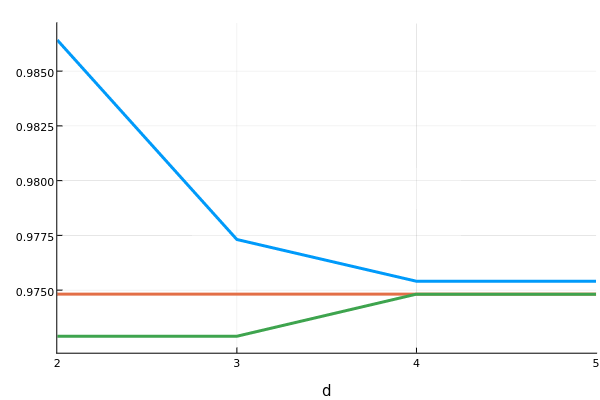
\includegraphics[width=\textwidth]{../../latex/images/PEDJ_zoom.png}
  \end{subfigure}
  \caption{Result of \exemref{run4}. The SOS UB is the upper bound found by \progref{primal} and the SOS LB is obtained from this upper bound the guarantee given in \cororef{mix}. The value $d$ of horizontal axis corresponds to using polynomials of degree $2d$. The right figure is a zoom of the left figure.}
  \label{fig:pedj}
\end{figure}



\subsection{Improving the automaton-dependent bounds}
Summarizing our results above,
after solving Program~\ref{prog:primal}, we obtain an upper bound on
the CJSR and a lower bound thanks to Corollary~\ref{coro:mix}.
Running Algorithm~\ref{algo:prodl} provides lower bounds that we can
compute if the sequence produced is periodic and this lower bound will
always be at least as high than the lower bound produced by
Theorem~\ref{theo:second}.

In this subsection we show that there is another way to improve the lower
bound provided by Theorem~\ref{theo:second} using the dual solution.
The improved lower bound will never be higher than the bound provided by
Algorithm~\ref{algo:prodl} but it only requires checking which dual values are zero
so it almost does not require any computation.
This lower bound is provided by the \theoref{fifth} which is a
generalization of \cite[Theorem~3.10]{philippe2016stability}.


\begin{definition}
  Consider \defAGe{}.
  Given a solution $\pmu$ of \progref{dual},
  we denote
  \[ \Arcs_{\pmu} = \{\, e \in \Arcs \mid \pmu_e \neq 0 \,\}. \]
  We define the graph $\G_{\pmu}(\Nodes,\Arcs_{\pmu})$ using this set of \arcs{}.
\end{definition}

\begin{theorem}
  \label{theo:fifth}
  Consider \defAG{} and a positive integer $d$.
  If $(\pmu, \gamlb)$ is a feasible solution of \progref{dual}
  then
  \[ \rho(\Adj(\G_{\pmu}))^{-\frac{1}{2d}} \gamlb \leq \cjsr \]
  where $A(\G_{\pmu})$ is the adjacency matrix of $\G_{\pmu}$.
  \begin{proof}
    For any edge $e \in \Arcs$ such that $\pmu_e = 0$, removing this
    edge does not violate any dual constraint \eqref{eq:dual1}.

    Using Theorem~\ref{theo:fourth} once we have removed all these
    edges and taking the limit $l \to \infty$ we obtain the result.
  \end{proof}
\end{theorem}

\begin{myrem}
  Note that it is not true that $\G_{\opt{\pmu}_{d_2}} \subseteq \G_{\opt{\pmu}_{d_1}}$ when
  $d_2 \geq d_1$ and $\pmu_{d_1}$ (resp. $\pmu_{d_2}$) is an optimal solution of \progref{dual}
  with polynomials of degree $2d_1$ (resp. $2d_2$).
  Indeed, as we have seen with Example~\ref{exem:run4} the dual
  variables of \arcs{} that were needed to have an s.m.p. are zero
  for $2d < 10$ so preventing Algorithm~\ref{algo:prodl} to choose
  these \arcs{} even for $l > 1$ prevents it to find the s.m.p. for
  $2d < 10$.
\end{myrem}

